
Let $x \neq y \in [0,1]$. Define the two-point distribution (\href{https://de.wikipedia.org/wiki/Zweipunktverteilung}{\enquote{Zweipunktverteilung}}) $T_{p,x,y}$, as the distribution that takes on value $P(X=x)=p$, $P(X=y) = 1-p$. 

Given a two-point distribution with points $x \neq y \in [0,1]$, that is a probability distribution that takes on values.

The mean is, which represents the overall connection probability,
\[
\E(\cdot) = \mu = px + (1-p)y.
\]
Given $\mu$,$x$ and $y$, the probability $p$ calculates as
\begin{align}
  p = \frac{c-y}{x-y}. \label{eq:bd1}
\end{align}
We can easily compute the expected overrepresentation in the network:
\begin{align}
  \sigma = \frac{p x^2 + (1-p) y^2}{\mu^2} \label{eq:bd2}
\end{align}
Using \eqref{eq:bd1}, equation~\eqref{eq:bd2} can be reduced to three parameters. It's the question which parameters and how to explore the parameter space.

For example, one can write:
\[
\sigma = \frac{x+y}{\mu} - \frac{xy}{\mu^2}.
\]
See: \href{https://www.wolframalpha.com/input/?i=Simplify[%28%28%28c-y%29%2F%28x-y%29%29*x^2%2B%281-%28%28c-y%29%2F%28x-y%29%29%29*y^2%29%2Fc^2]}{Wolfram Alpha}.

\begin{figure}[h!]
\centering
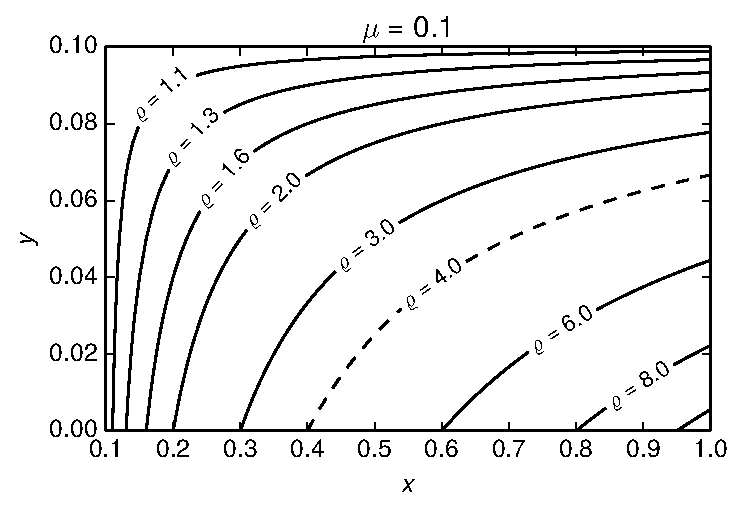
\includegraphics[width=0.6\textwidth]{../lab/two_point_distribution/contour_plot.png}
\caption{Contour plot shows different pairings}
\end{figure}



